\chapter{Antecedentes}
\label{chap:antecedentes}

\drop{A}{ctualmente}, las empresas se encuentran en una fase que se denomina como de <<digitalización>> o <<transición digital>>. Esto, unido a las posibilidades que ofrece la nube y los avances en la tecnología, permite una mayor expansión de estas, a la par que requieren de servicios innovadores para afrontar esta transición, continuando su actividad empresarial. Uno de estos servicios es el llamado \acf{DaaS}, que permite la <<ultramovilidad>>, mejorando el entorno laboral de los trabajadores. No obstante, como se ha nombrado anteriormente, para poder ofrecer dicho servicio a una gran cantidad de personas de manera simultánea, se hace necesaria la virtualización, una tecnología que ha ido evolucionando a lo largo de los años.


\section{Introducción a la virtualización}
La virtualización no es sino una tecnología que permite la creación de nuevos recursos virtuales dentro de otros recursos físicos ya existentes. Es decir, mientras la máquina física disponga de capacidad de cómputo suficiente, esta podrá albergar diferentes máquinas o recursos virtuales dentro de ella, de manera que se evite la necesidad de disponer de múltiples máquinas adicionales. Esto puede aportar diferentes ventajas, donde una de las más importantes es la de aprovechar todos los recursos disponibles, aumentando la eficiencia final. Atendiendo a la Figura \ref{fig:ejemplo_virtu}, en el caso de disponer de un servidor de correo, otro para la página web y otro para aplicaciones (todos ellos en su manera tradicional, sin virtualizar), es posible crear dos servidores virtuales dentro del primero donde uno continúe realizando las tareas iniciales y el segundo se encargue de las tareas que antes estaban asignadas al tercero. De esta manera, incluso se puede llegar a prescindir de máquinas físicas, lo que derivaría en un ahorro energético. No obstante, ha sido en los últimos años cuando esta tecnología se ha comenzado a desarrollar lo suficiente como para poder ser aprovechada y explotada a mayor escala.

\clearpage

\begin{figure}
    \centering
    \begin{minipage}{.5\textwidth}
        \centering
        
\includegraphics[width=0.9\linewidth]{figures/images/serv_s_virt.png}
    \end{minipage}%
    \begin{minipage}{.5\textwidth}
        \centering
        
\includegraphics[width=0.9\linewidth]{figures/images/serv_c_virt.png}
    \end{minipage}
    \caption{Comparación de servidores con y sin virtualización}
    \label{fig:ejemplo_virtu}
    \source{\url{https://www.redhat.com/es/topics/virtualization/what-is-virtualization}}
\end{figure}

Aunque los términos de <<virtualización>> o <<máquina virtual>> (\acs{MV}) se encuentren muy extendidos hoy en día, fue la empresa IBM la que, en la década de los años 60, desarrolló un sistema que permitiera disponer de particiones lógicas a partir de las supercomputadoras existentes en aquella época con el principal objetivo de realizar múltiples tareas de manera simultánea. Por aquel entonces, el \acf{SO} que utilizaba IBM se denominaba <<supervisor>> que, con la virtualización, pasó a llamarse <<hipervisor>>, ya que era capaz de manejar varios SSOO \cite{josemariagris2012}. Esto se denominó como <<virtualización de plataforma>> \cite{mtimjones2011}.

A pesar de sus posibilidades, la virtualización no comenzó a ser ampliamente adoptada hasta la década de los 90, donde las empresas solían utilizar recursos de un único proveedor. Debido a esto, al renovar estos por otros de diferentes proveedores, la utilización del hardware comenzaba a ser ineficiente  y la virtualización era una tecnología que solventaba estas carencias, además de reducir costes de compra, instalación, refrigeración y mantenimiento \cite{redhat}. Utilizando la herramienta  <<Google \textit{Trends}>>, es posible ver la evolución en las búsquedas que ha tenido el término <<virtualización>> desde el 01-01-04 hasta el 01-09-19. La Figura \ref{fig:evo_virt} muestra una tendencia ascendente hasta 2009, donde alcanza un máximo, para disminuir gradualmente hasta mantenerse en los valores estables en los que se encuentra actualmente.

\begin{figure}[h]
  \centering
  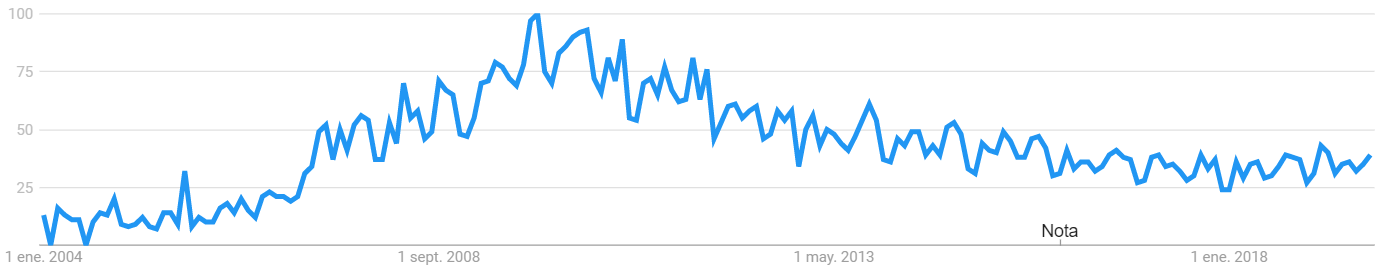
\includegraphics[width=0.9\linewidth]{figures/images/evo_virt.PNG}
  \caption{Evolución <<virtualización>>}
  \label{fig:evo_virt}
\end{figure}

\clearpage

\section{Funcionamiento de la virtualización}
El llamado <<hipervisor>> que se ha mencionado anteriormente es un elemento indispensable en la virtualización, puesto que es el que realiza la tarea de separación de los recursos físicos y los virtuales, encargándose de su gestión para que los primeros sean accesibles por los segundos (Figura \ref{fig:hipervisor}). De esta manera, los usuarios interactúan con una máquina que se encuentra virtualizada, aunque tengan la sensación de estar utilizando una física al uso. Esta puede ser, además, migrada a otros servidores, puesto que se trata de una virtualización aislada e independiente del entorno de ejecución. Por tanto, cuando un usuario interacciona con la máquina virtual, el hipervisor es el que se encarga de transmitir las órdenes al sistema físico \cite{redhat}.

\begin{figure}[h]
  \centering
  
\includegraphics[width=0.32\linewidth]{figures/images/hipervisor.png}
  \caption{Situación del hipervisor}
  \label{fig:hipervisor}
  \source{\url{https://www.redhat.com/es/topics/virtualization/what-is-virtualization}}
\end{figure}

\section{Tipos de virtualización}
Aunque IBM introdujo la virtualización de plataforma en los años 60, actualmente existen otras formas de virtualización \cite{redhat}:

\begin{itemize}
    \item \textbf{Virtualización de los datos}. La principal utilidad de este tipo de virtualización es la de tratar diferentes fuentes de datos como una única fuente (Figura \ref{fig:data_virt}).
    
        \begin{figure}[h]
          \centering
          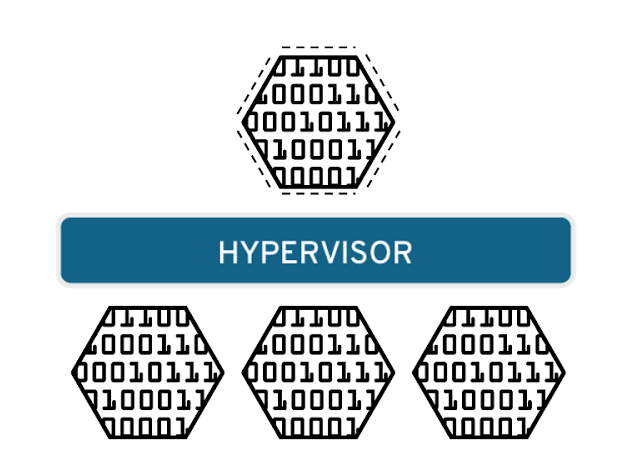
\includegraphics[width=0.3\linewidth]{figures/images/data_virtualization.png}
          \caption{Virtualización de datos}
          \source{\url{https://www.redhat.com/es/topics/virtualization/what-is-virtualization}}
          \label{fig:data_virt}
        \end{figure}
        
    \clearpage
        
    \item \textbf{Virtualización de los escritorios}. Mediante esta virtualización, es posible entregar una cierta cantidad de escritorios <<simulados>> a partir de una o varias máquinas físicas (Figura \ref{fig:desktop_virt}).
    
        \begin{figure}[h]
          \centering
          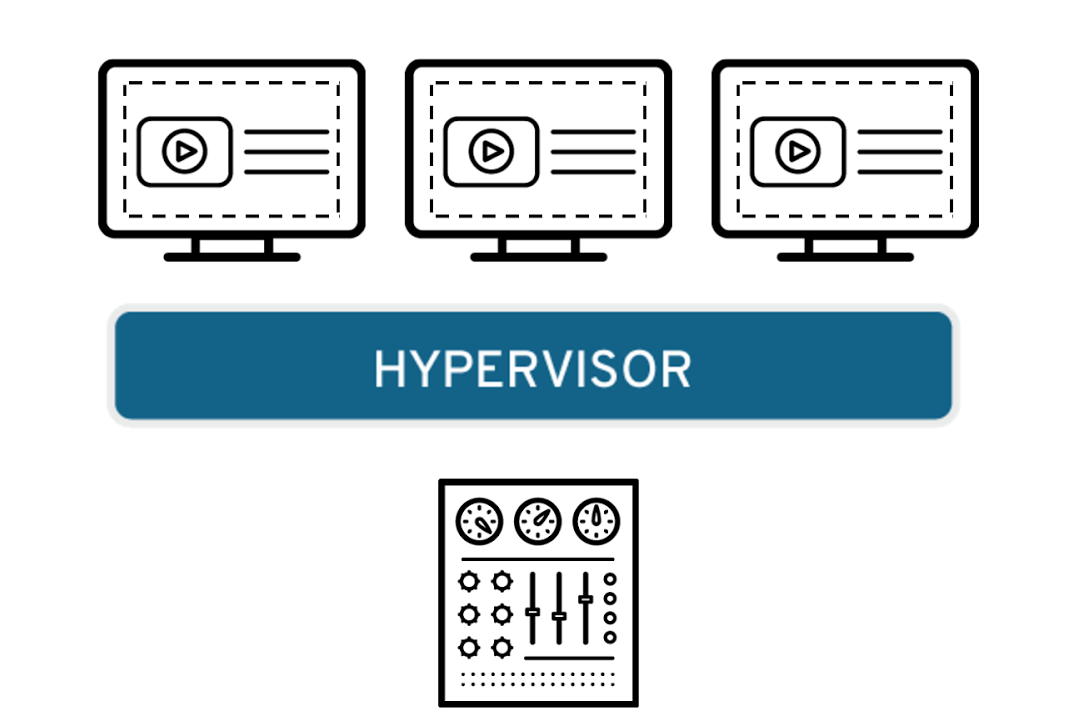
\includegraphics[width=0.3\linewidth]{figures/images/desktop_virtualization.png}
          \caption{Virtualización de escritorio}
          \source{\url{https://www.redhat.com/es/topics/virtualization/what-is-virtualization}}
          \label{fig:desktop_virt}
        \end{figure}
        
    \item \textbf{Virtualización de los servidores}. Este tipo de virtualización consiste en dividir un servidor en otros virtuales, de manera que sus recursos sean aprovechados de una manera más eficiente, como se ha mencionado anteriormente en un ejemplo (Figura \ref{fig:server_virt}).
    
        \begin{figure}[h]
          \centering
          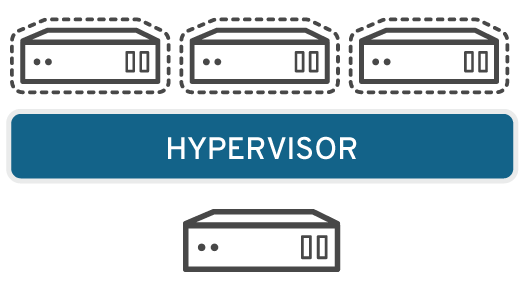
\includegraphics[width=0.3\linewidth]{figures/images/server_virtualization.png}
          \caption{Virtualización de servidores}
          \source{\url{https://www.redhat.com/es/topics/virtualization/what-is-virtualization}}
          \label{fig:server_virt}
        \end{figure}
        
    \item \textbf{Virtualización del sistema operativo}. A partir de esta virtualización, es posible ejecutar un sistema operativo completo de manera paralela en una misma máquina. Esta virtualización es una de las más conocidas, ya que es la que implementan programas como VirtualBox, VMware o Parallels Desktop (Figura \ref{fig:os_virt}).
    
        \begin{figure}[h]
          \centering
          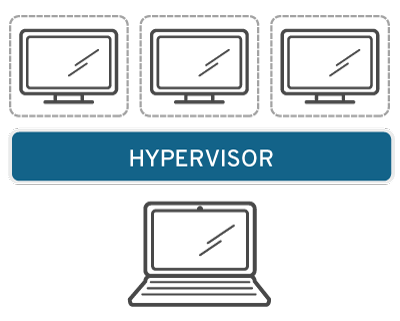
\includegraphics[width=0.3\linewidth]{figures/images/os_virtualization.png}
          \caption{Virtualización de sistema operativo}
          \source{\url{https://www.redhat.com/es/topics/virtualization/what-is-virtualization}}
          \label{fig:os_virt}
        \end{figure}
        
    \clearpage
    
    \item \textbf{Virtualización de las funciones de red}. El principal cometido de este tipo de virtualización es el de separar las funciones clave de una red para distribuirlas entre entornos. De esta manera, las funciones específicas se asignan a un entorno específico, reduciendo los componentes físicos (Figura \ref{fig:net_virt}).
    
        \begin{figure}[h]
          \centering
          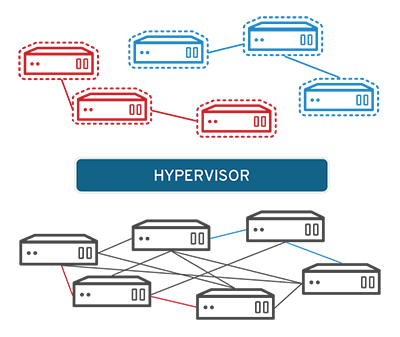
\includegraphics[width=0.3\linewidth]{figures/images/network_virtualization.png}
          \caption{Virtualización de funciones de red}
          \source{\url{https://www.redhat.com/es/topics/virtualization/what-is-virtualization}}
          \label{fig:net_virt}
        \end{figure}
\end{itemize}

Por tanto, la virtualización, en sus diferentes variantes, ofrece diversas ventajas, como la de unificar datos, utilizar los recursos con una mayor eficiencia o separar las funciones de red clave de las específicas. Esto hace que la implementación de esta y otras tecnologías posea un carácter llamativo, lo que deriva en un mayor uso de las \acf{TI} que, a su vez, impulsa dicha implementación, representando un ciclo de mejora e innovación. Este ciclo posee una gran importancia en la actualidad tanto en empresas e instituciones en general como en las universidades en particular, donde la percepción de la innovación y el hecho de utilizar recursos novedosos y cada vez más tecnológicos podría aumentar el interés por parte de los potenciales alumnos, además de proporcionar un modelo docente diferenciador con respecto a otras universidades. Por tanto, lo anterior podría traducirse en un aumento en el número de matriculados, impulsando las universidades que adopten nuevas tecnologías y modelos docentes.

\section{Las \acs{TI} en las universidades}
Cerrando el foco sobre el ámbito universitario, entorno sobre el que se desea que la empresa desarrolle su actividad, se ha utilizado el último informe de la \acf{CRUE} relativo al análisis de las \acf{TIC} en las universidades españolas, publicado en octubre de 2017 \cite{universitic2017}.

En su resumen ejecutivo, destacan algunos comentarios que sobresalen por encima del resto, puesto que resultan de gran relevancia para el trabajo que se plantea realizar. <<La apuesta de las universidades por las \acs{TI} como soporte y apoyo a la docencia ha alcanzado niveles de saturación>>. Además, se indica que servicios como la docencia virtual se encuentran implantados en la práctica totalidad de las universidades que participaron en el estudio.

\clearpage

<<Cada vez las universidades ponen menos equipamiento genérico a disposición de los estudiantes [...] pero aumentan los servicios para facilitar el uso de sus propios equipos>>. Se incluye en esta parte un aumento del 13\% en el catálogo de aplicaciones virtuales de escritorio. Esto refuerza la afirmación anterior de que la implementación de la virtualización, entre otros aspectos, posee un carácter atractivo para, en este caso, las universidades. Por otra parte, se indica que alrededor del 85\% de las universidades han considerado ofrecer cursos \acf{MOOC}, que podrían llegar a hacer uso de la mencionada virtualización. También se desprende del informe la preocupación de las universidades con respecto al tratamiento de la información, ya que <<es destacable el interés [...] por los aspectos de seguridad y los indicadores vinculados al \acf{ENS}>>. Esto hace visible que la información, hoy en día, es uno de los activos más valiosos de los que puede disponer una entidad, empresa o institución y debe preocuparse por tareas tan importantes como el correcto tratamiento y almacenamiento.

El informe menciona varios <<temas emergentes>>, que son los considerados como de reciente incorporación y que, por tanto, aún poseen un bajo valor aunque con un crecimiento considerable. Entre dichos temas, cabe destacar el primero de ellos: escritorios virtuales. Este indicador fue incorporado en el informe desarrollado en 2015 y, en el informe de 2017, se señala que se ha duplicado la cantidad de configuraciones software que se ofrecen en el catálogo de escritorios y aplicaciones virtuales. Asimismo, la cantidad de \acs{MOOC} se habría duplicado igualmente desde 2015, fruto del mencionado interés por parte del 85\% de las universidades por ofrecer este tipo de cursos.

De la misma manera, existen <<temas consolidados>>, considerados como indicadores con un alto valor. Uno de ellos son los <<servicios \acs{TI} de soporte a la docencia>>, con una media del 90,38\% del total de servicios incluidos en el catálogo, lo que representa que prácticamente el total de los servicios que ofrecen las universidades son de este tipo. Esto, unido a que el 83\% de las aulas cuentan, como mínimo, con conexión a Internet y proyector, refuerza la idea de <<transición digital>> que se ha mencionado anteriormente.

La Figura \ref{fig:infounitic} muestra una infografía que se encuentra en el informe, resumiendo los indicadores más importantes y aspectos más destacados de este. Por tanto, teniendo en cuenta todo lo expuesto anteriormente y el estado actual en el que se encuentra el desarrollo de las tecnologías y, en concreto, la de virtualización, es posible observar cómo se está virando hacia una sociedad que ofrece servicios cada vez más digitales. En consecuencia, se proporciona un sector que puede ser de gran interés para las empresas que pretendan acceder a este para ofrecer servicios novedosos e innovadores que satisfagan las necesidades de las universidades por ofrecer una mayor calidad de enseñanza.

\begin{figure}[h]
  \centering
  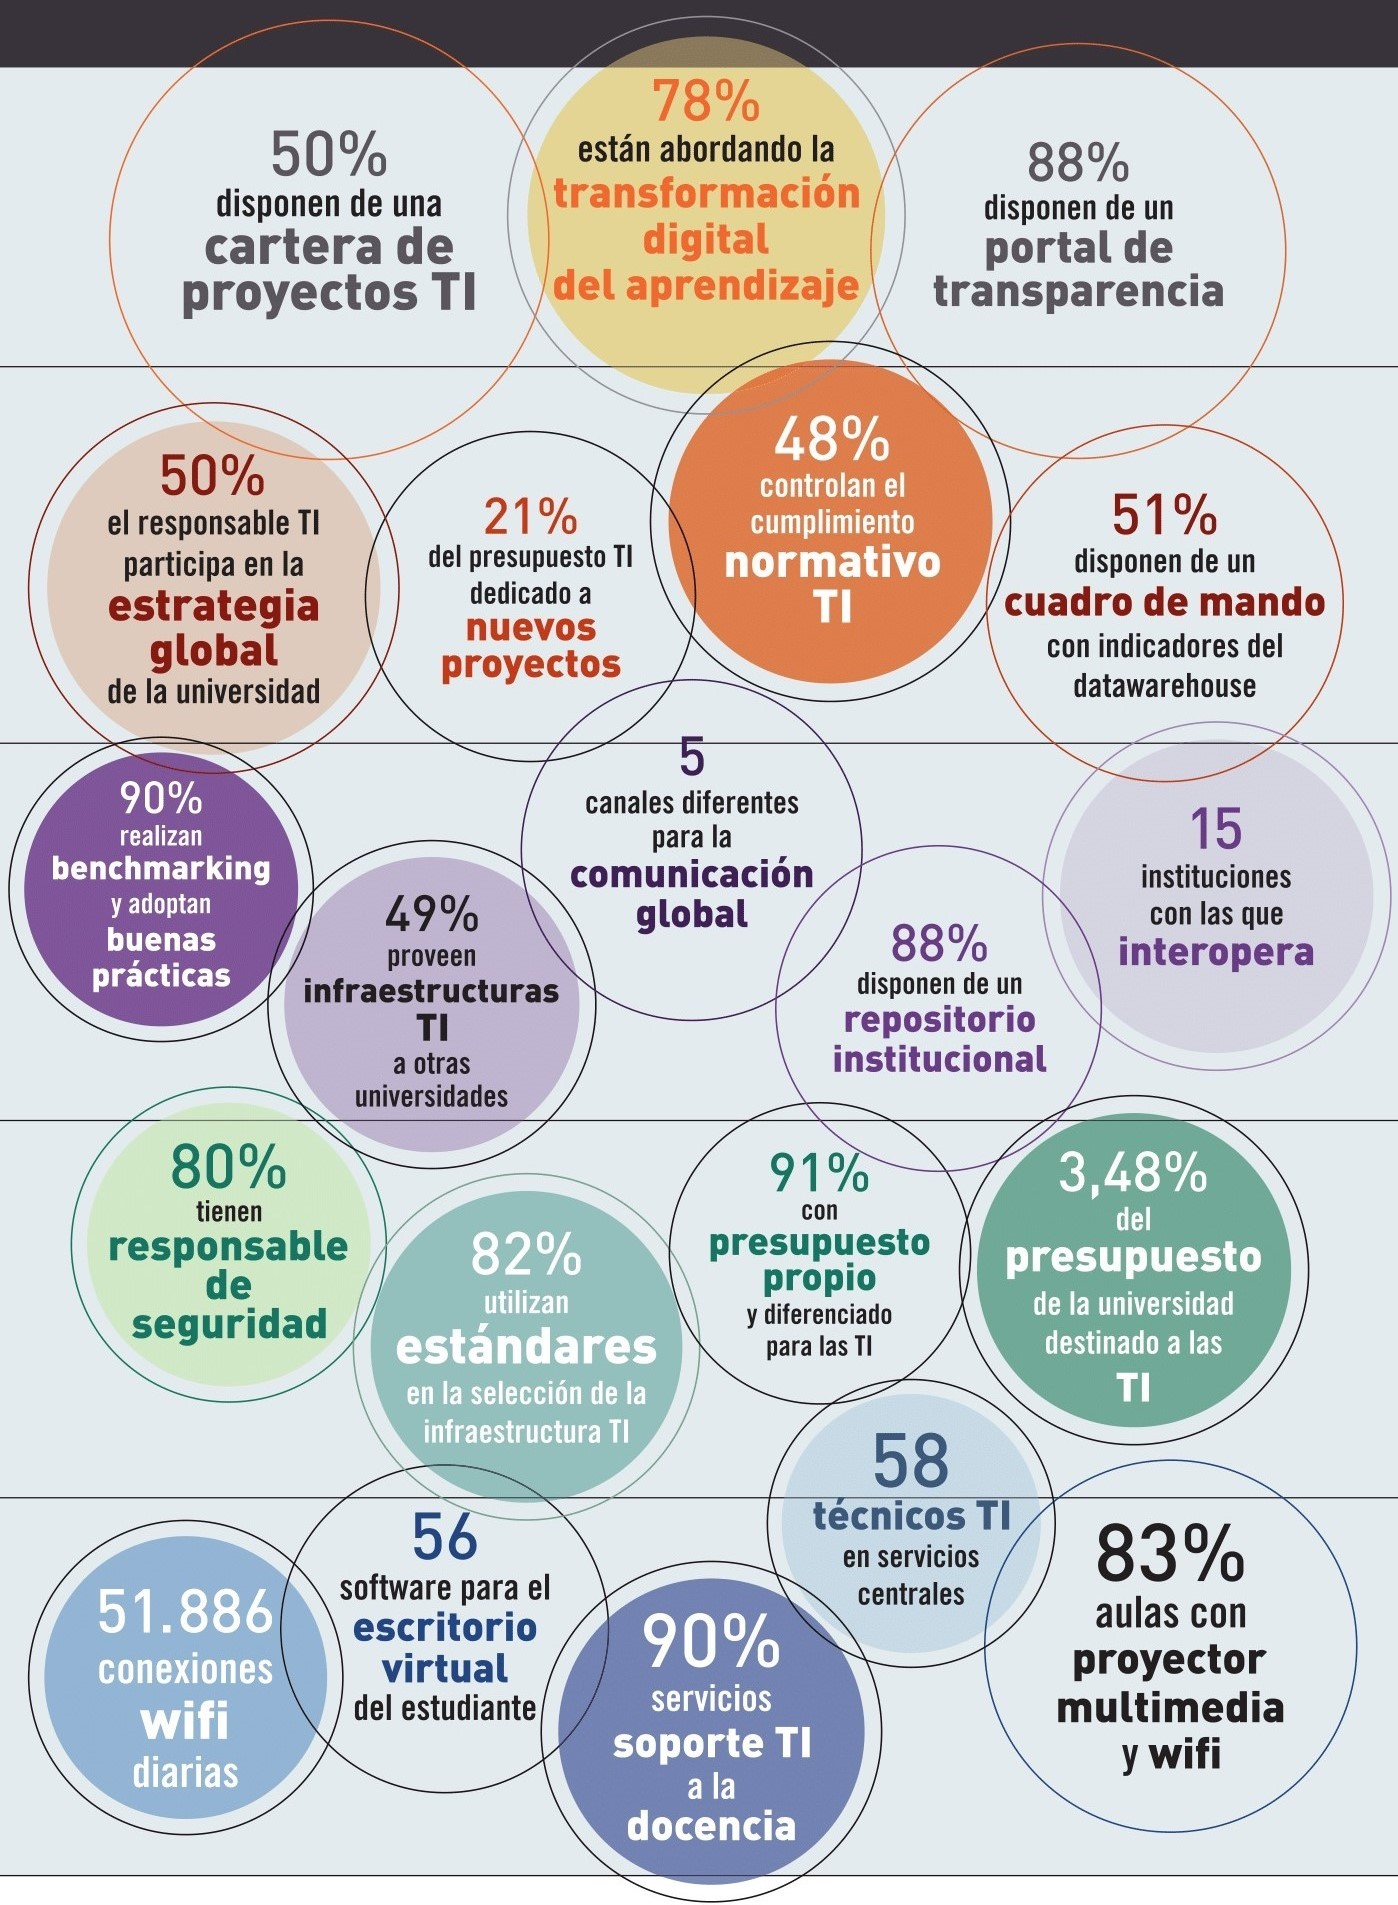
\includegraphics[width=0.9\linewidth]{figures/images/resumen_universitic.jpg}
  \caption{Infografía Universitic}
  \source{\url{http://tic.crue.org/wp-content/uploads/2018/03/UNIVERSITIC-2017.pdf}}
  \label{fig:infounitic}
\end{figure}

%No obstante, este servicio no se ha presentado siempre de la misma manera, sino que ha ido evolucionando con el tiempo y, con este, han surgido nuevas empresas dedicadas a satisfacer las nuevas demandas para ofrecer este tipo de servicio. Este capítulo estará enfocado a realizar un análisis de la evolución de estos servicios y empresas, junto con las ventajas que ofrece cada una, de manera que se pueda tener una visión más abierta.

% Local Variables:
%  coding: utf-8
%  mode: latex
%  mode: flyspell
%  ispell-local-dictionary: "castellano8"
% End:
